\documentclass{ifacconf}

\usepackage{natbib}            % you should have natbib.sty
\usepackage{graphicx}          % Include this line if your
                               % document contains figures,
\usepackage{epsfig}            % or this line, depending on which
\newcommand{\squeezeup}{\vspace{-3.0mm}}
%\usepackage[dvips]{epsfig}    % or this line, depending on which
                               % you prefer.
% predefined environments
%\begin{thm} ... \end{thm}		% Theorem
%\begin{lem} ... \end{lem}		% Lemma
%\begin{claim} ... \end{claim}	% Claim
%\begin{conj} ... \end{conj}	% Conjecture
%\begin{cor} ... \end{cor}		% Corollary
%\begin{fact} ... \end{fact}	% Fact
%\begin{hypo} ... \end{hypo}	% Hypothesis
%\begin{prop} ... \end{prop}	% Proposition
%\begin{crit} ... \end{crit}	% Criterion

\usepackage{enumitem}

\begin{document}

\begin{frontmatter}

\title{Cooperative Autonomy of Multiple Solar-Powered Thermaling Gliders
\thanksref{footnoteinfo}}

\thanks[footnoteinfo]{The project has been supported by the NPS Consortium for
Robotics and Unmanned Systems Education and Research, the Army Research Lab,
and "The Multidisciplinary Studies Support for USMC Expeditionary Energy
Office" program.}

\author[First]{Nahum Camacho,}
\author[Second]{Vladimir N. Dobrokhodov, Kevin D. Jones,}
%\author[Third]{Isaac I. Kaminer}

\address[First]{Graduate student at the Department of Mechanical and Aerospace Engineering,
Naval
Postgraduate School, Monterey, CA 93943 USA (e-mail: ncamacho@nps.edu)}
\address[Second]{Research Associate Professors at the Department  of Mechanical and Aerospace
Engineering, Naval Postgraduate School, Monterey, CA 93943 USA (e-mail: {vndobrok,
kdjones}@nps.edu)}
%\address[Third]{Professor at the Department  of Mechanical and Aerospace Engineering, Naval
%Postgraduate School, Monterey, CA 93943 USA (e-mail: kaminer@nps.edu)}


\begin{keyword}                           % Five to ten keywords, chosen from the IFAC
cooperative control; solar energy; convective lift; autonomous soaring; UAV.
\end{keyword}                             % keyword list or with the
                                          % help of the Automatica
                                          % keyword wizard


\begin{abstract}                          % Abstract of not more than 250 words.
This paper presents a review of the multidisciplinary approach to the
design of a fleet of cooperative gliders capable of extended endurance
operation. The flock of autonomous gliders is able to harvest energy from
the environment, both through photo-voltaic energy generation and through
exploitation of natural convective lift in the surrounding air, and act
cooperatively to meet mission requirements and to share knowledge of the
local environment. The paper begins with a brief overview of the
total-energy approach required for such a feat, along with a short
description of key system components and the principal technologies. This
is followed by details of the evolution of a previously-developed
architecture that supported autonomous thermaling, to an architecture that
considers the total-energy budget in all flight segments, and utilizes the
cooperative flight to maximize the cumulative energy capture while
simultaneously meeting mission objectives.
\end{abstract}

\end{frontmatter}

\section{Introduction}
\squeezeup
%Imagine a large team of gracefully soaring autonomous gliders, instrumented with sensors
%capable of detecting convective air currents in the environment, and equipped with
%high-efficiency solar arrays which are seamlessly embedded into the wings to replenish
%the electrical energy in the batteries that power the avionics. The gliders are launched
%from a remote location and assigned to provide, for example, wide area network coverage
%or to serve as pseudo Low-Earth-Orbit satellites to aid in fighting forest fires or to
%support border protection. The gliders reach the area of operation and remain there
%unattended for an extended period of time, perhaps up to a year. When a need for
%maintenance arises the distributed intelligent algorithm reconfigures the team of gliders
%and calls back the aircraft in need of service. In turn, when a substitute or serviced
%aircraft returns, the same algorithm reconfigures the team to accept the new player.
%Members of the flock can either operate in a distributed fashion or fly together in a
%suitable formation to provide a more focused capability. The latter may include
%cooperative distributed sensing to achieve a desired sensor resolution, tracking of
%weather formations, border patrol, and many other tasks that are currently provided by
%much larger, heavier, and more expensive systems.

%
%Despite current advances in many key technology areas associated with unmanned systems -
%advances which have resulted in significant reductions in Size, Weight and Power (SWAP)
%of individual system components, the ability to stay aloft for extended periods (days,
%months, years) remains a daunting task. Larger UAVs such as Predator and Global Hawk (see
%\cite{Best:2005} have broken the 24-hour mark, but burning fossil fuels, they are still
%limited by the size of the gas tanks they can carry. This type of larger aircraft can
%only meet the $24/7$ continuous coverage goal by using several aircraft that take turns
%on station, and each aircraft requires a large team of humans to operate, amounting to a
%very large footprint and cost. While the capability they provide is enormous, the
%operational cost for continuous coverage is prohibitive, and limits their use primarily
%to high-value missions.

%
%In order to reach the $24/7$ goal with a single asset, one must depart from the need for
%fossil fuels, and absorb energy from the environment. Historically, this has typically
%been done using photo-voltaics to generate electricity for propulsion, avionics and
%sensors. Projects like this date back to the 1970s (cite Noth history), and have
%demonstrated various levels of success. However, in order to carry a payload with a
%significant mass and power requirement, the required size of the vehicle has been driven
%to extremes in order to satisfy the stringent power budget. The size and complexity of
%these large platforms drives the cost very high, and the fragility of the structure,
%pushed to the limits by size and weight constraints, has resulted in the catastrophic
%destruction of many of these experimental platforms when they experienced mild turbulence
%in the atmosphere.

%
%There have been several projects that have sought to capitalize on convective lift in the
%environment to offset or remove the need for propulsion (cite refs from Hambling
%article), extending endurance to the limits of the battery capacity the aircraft can
%carry and the energy requirements of the avionics and payload. A challenge for these
%vehicles revolves around locating the regions of advantageous lift. The recent
%development by~\cite{AKlass_JGCD:2012,AKlass_CDC:2012} demonstrated that teams of
%aircraft working cooperatively could improve the probability of success by splitting up
%the search task and sharing location data for regions of lift. Combining the ability to
%exploit natural lift in the environment with photo-voltaic energy production, the
%vehicles should be able to stay aloft $24/7$, while still having enough additional energy
%to support the weight and power of meaningful payloads.

%
%This project proposes a paradigm shift, away from single, large, high-dollar assets,
%toward a large fleet of smaller, very inexpensive assets. Each of the small assets has
%limited payload capacity, but the large number of assets allows for a variety and wide
%distribution of sensors over the area of operation. Loss of a single vehicle form a flock
%of 100, results in the loss of 1\% of your sensing capability and very little monetary
%loss, compared to the single large asset where any loss is a total loss.

One of the most critical limiting factors impacting effective collaborative
autonomy today is the lack of range and endurance that are typical in most of
the existing autonomous aircraft; see a comprehensive review in
\cite{NAC:2005}.
%
%Numerous futuristic ideas and concepts will not be implemented in real life
%solely due to this reason. Until $R\&D$ community realizes that the energy
%onboard (of either a single or a flock of agents) and the mission objectives
%are equally important metrics of the mission management (planning and
%execution), and finds a way of solving this challenge, there will not be
%revolutionary advances made in the area of persistent intelligent
%collaborative autonomy.
%
Despite almost two decades of significant advances in low-power and
high-performance microelectronics development including CPUs, sensors,
actuators, and communication circuits (see~\cite{Singh:2010}), the only task
addressed was to lower the power consumption and to reduce the pace of energy
expenditures. In turn, the progress in energy renewable technologies has also
been advancing fast, especially in the flight-relevant areas of solar
photovoltaics (PV) (\cite{Hamakawa:2004}) and electro-chemical battery
technologies, see \cite{Tarascon:2001}. Yet, the balance of energy use and
the regenerated energy income has not been met. Since the loss of energy is
unavoidable due to the limited efficiency of energy conversion, storage, and
transmission, the traditional mission duration will always be limited.
However, coupling these existing advances with convective air (thermal)
soaring capabilities and novel approaches in the cooperative mission planning
and execution can not only further reduce the rate of loss of onboard energy,
but can also result in energy increase during the autonomous mission; this
capability is not readily available today in any of the available
technologies, see~\cite{Martinez:2008}, and
\cite{Nonami:2013}.
%\cite{Siciliano:2008},
%Despite the complexity of the energy-management task, the practical solutions
%of the extended range and duration flight do exist in nature. Millions of
%years of evolution enable a number of families of birds for very long
%duration flights. While the fundamentals of flight are the same, the
%effective energy management principles during the flight do differ. One of
%the most extraordinary birds capable of the long duration flight is the
%bar-tailed godwit, a large, streamlined shorebird, that performs a non-stop
%across the ocean flight, see\cite{USGS:2007}, of more than eight days over a
%distance of 7,200 miles; the distance equivalent of making a round-trip
%flight between New York and Paris without ever touching down. Remarkably,
%some birds can remain aloft for years at a time; the swift, for example,
%spends nearly its entire life in the air while landing only to breed. Along
%with many other animals (for example dolphins, whales), swifts evolved to be
%able to put one side of their brain to sleep at a time, so that they can
%sleep in the air while not actually being unconscious,
%see~\cite{Lapierre:2007}. What is common among these examples is not only the
%evolved capability of the high efficiency flight, but also the unique ability
%to manage energy that is implemented by both the optimal energy expenditures
%and energy harvesting.
%
%Another example is the albatross that can fly around the world with little or
%no flapping of their wings, see~\cite{Richardson:2011}.

Considering the state of the art in aerial robotics (algorithmic support,
instrumentation, size weight and power constraints), it is our belief that
the best approach to enable long duration flight would combine the
collaborative mission management with the energy harvesting and onboard
storage. \emph{Collaboration} is the first key capability that spans across
every element of the mission as it enables effective search for available
energy sources. Most of the available energy sources can be detected by
autonomous vehicles equipped with appropriate sensors. Thus, multiple agents
would have much better chances of finding ''free energy`` when cooperating
and sharing their findings. Second, the operational utility of multiple
agents equipped with complementary sensors is superior to the capability of
an individual agent. Finally, robustness of the collaborative mission
execution is significantly higher because partial loss of a subset of the
vehicles does not lead to the loss of entire flock capability. \emph{Energy
harvesting and storage} is the second complementary enabler of long endurance
flight that allows for the accumulation of energy. The feasible methods of
energy extraction in aerial application include the solar PV and airflow
soaring; the soaring can be based on the convective air (thermaling) or wind
shear energy extraction. While the PV boost can be achieved only during the
daylight, the extraction of power of surrounded moving air can be utilized
even during the nighttime. The combination of harvesting and storage is the
ultimate solution for the "eternal`` flight.

%%%Isaac%%%
%Energy storage devices. What is the metric of measuring the efficiency of
%batteries. Energy density? Give a clear picture of the trend in energy
%density or other metric over the next 10-20 years to better motivate the
%research in cooperative energy harvesting and storage technologies.


%enhancing mission performance can be
%achieved by implementing the energy harvesting-storage and collaboration
%capabilities onboard of multiple autonomous solar-powered and thermal-soaring
%gliders. Thus,
Therefore, it is envisioned that the triplet of (\emph{\textbf{i}}) mission management,
(\emph{\textbf{ii}}) energy harvesting-storage and (\emph{\textbf{iii}})
collaboration builds the fundamental architecture of future energy enhanced
autonomy.
%
%This architecture should be based on the distributed execution of the
%following individual and distributed platforms' algorithms:
%\begin{itemize}[leftmargin=0.35cm]
%%%%%%%%%%%%
% \item Individual glider:
% \begin{itemize}[leftmargin=0.25cm]
% \item Integration of prior knowledge of the operational environment into
%     effective collaborative search for energy;
% \item Identification of the inherent flying qualities of each glider and
%     detection of the environmental energy excess (convective thermal or
%     wind shear);
% \item Identification of parameterized mathematical models of energy
%     sources and estimation of their dynamic motion;
% \item Autonomous guidance to enable energy harvesting while in the
%     vicinity of an energy source;
% \item Optimization of solar energy gain and electrical energy storage
%     while in the thermal soaring flight;
% \item Sharing of the environment knowledge and the current state of
%     cumulative energy of each glider;
% \end{itemize}
%%%%%%%%%
%\item Flock of gliders:
%\begin{itemize}[leftmargin=0.25cm]
%  \item Distributed mission planning and cooperative control of the flock
%      as functions of mission objectives and the reported cumulative
%      energy of the flock; local feedback to the mission planner allows
%      for timely update and adjustment;
%  \item Cooperative estimation of the free energy density distribution in
%      the operational environment;
%  \item Adjustment of the scale of the mission (number and strategy of
%      multiple agents) defined by the rate of total energy expenditure.
%\end{itemize}
%\end{itemize}
The remainder of the paper briefly outlines the core ideas implemented to
date in autonomous thermaling. The section \ref{sec:IndAlgs} describes the
''individual gliders`` algorithms. The following section \ref{sec:CoopAlgs}
outlines the development of the collaborative autonomy algorithms. Section
\ref{sec:SimEnv} provides details of the developed high-fidelity simulation
environment used to verify the algorithms.
%The paper ends with a brief outline of the future development steps.

\section{ Algorithms of Individual Gliders}
\label{sec:IndAlgs} \squeezeup This section discusses the algorithms that run
online and enable \emph{identification of the flight dynamics} of the glider,
which are in turn used to \emph{detect the thermal updrafts}. When flying in
the updraft, the \emph{guidance algorithm} is engaged to enable the maximum
energy harvesting efficiency of the updraft's free energy, and on the other
hand \emph{estimates the updraft geometry and motion}, that are used to
georeference the updraft and share its utility properties (strength) across
the network of collaborative gliders.
%
%Besides the collaborative mission objective and an initial mission plan, the
%georeferenced map represents the formalized knowledge used in the
%collaborative mission replanning phase.
%
While in autonomous soaring mode, the \emph{electrical management} system
that consists of solar PV panels, batteries and the maximum peak power energy
tracking (MPPT) unit, supports the avionics and recharges the batteries
keeping them evenly balanced.\squeezeup

%At any given time each individual platform can be either in a mission-induced
%search or in a soaring modes. While the soaring mode is primarily defined by
%the energy gain objective, the mission-induced search mode is driven by the
%algorithm that combines the goals of the distributed mission and the need to
%search for energy sources in the environment.
%
%Development of these onboard components that enable optimal balancing of
%energy gain and mission objectives is the most promising direction of the
%current and future research.

\subsection{Electric Energy Management Subsystem}
\label{subsec:Electric}
\squeezeup

The project considers two sources of energy input into the system: PV and
atmospheric convection, and typically two methods of energy storage;
potential energy stored chemically in batteries and potential energy stored
via altitude. Obviously, for a given glider the electrical energy can be
translated into the potential gain of altitude that is critical at the
mission planning stage. This section describes the electrical half of that
system; electricity harvesting through PV conversion and energy storage in
rechargeable batteries.

While the electrical system architecture is conceptually well-understood, the
variation of physical and mechanical properties of PV panels and batteries
presents the most significant uncertainty, and thus poses the challenge for
the overall system design. Not only basic physical properties of all
components vary significantly, but also the same properties depend on the
mode of operation (e.g. discharge rate) and environmental parameters(e.g.
temperature). Thus, before the electrical system is integrated onboard it is
necessary to characterize mathematically the solar-powered energy generation,
storage, and the energy expenditure system, so that the particular uncertain
parameters could be identified on the ground and during the flight of a
particular glider platform. The need for online identification arises as the
properties of the system are expected to change over time.

%As an example of variation of system parameters, the following data represent
%the results of the discharge experiment performed with 2 different types of
%batteries at different discharge rates; the experiment utilized the Lithium
%polymer (LiPo) and the Lithium-Ion (LiIon) packs. Figure
%\ref{fig:Batt_v_vs_t} illustrates how voltage drops over the discharge cycle,
%a feature that is convenient for estimating remaining energy in the battery
%pack.
%%%%%%%%%%%%%%%%%
%\begin{figure}[thbp]
%  \centering
%  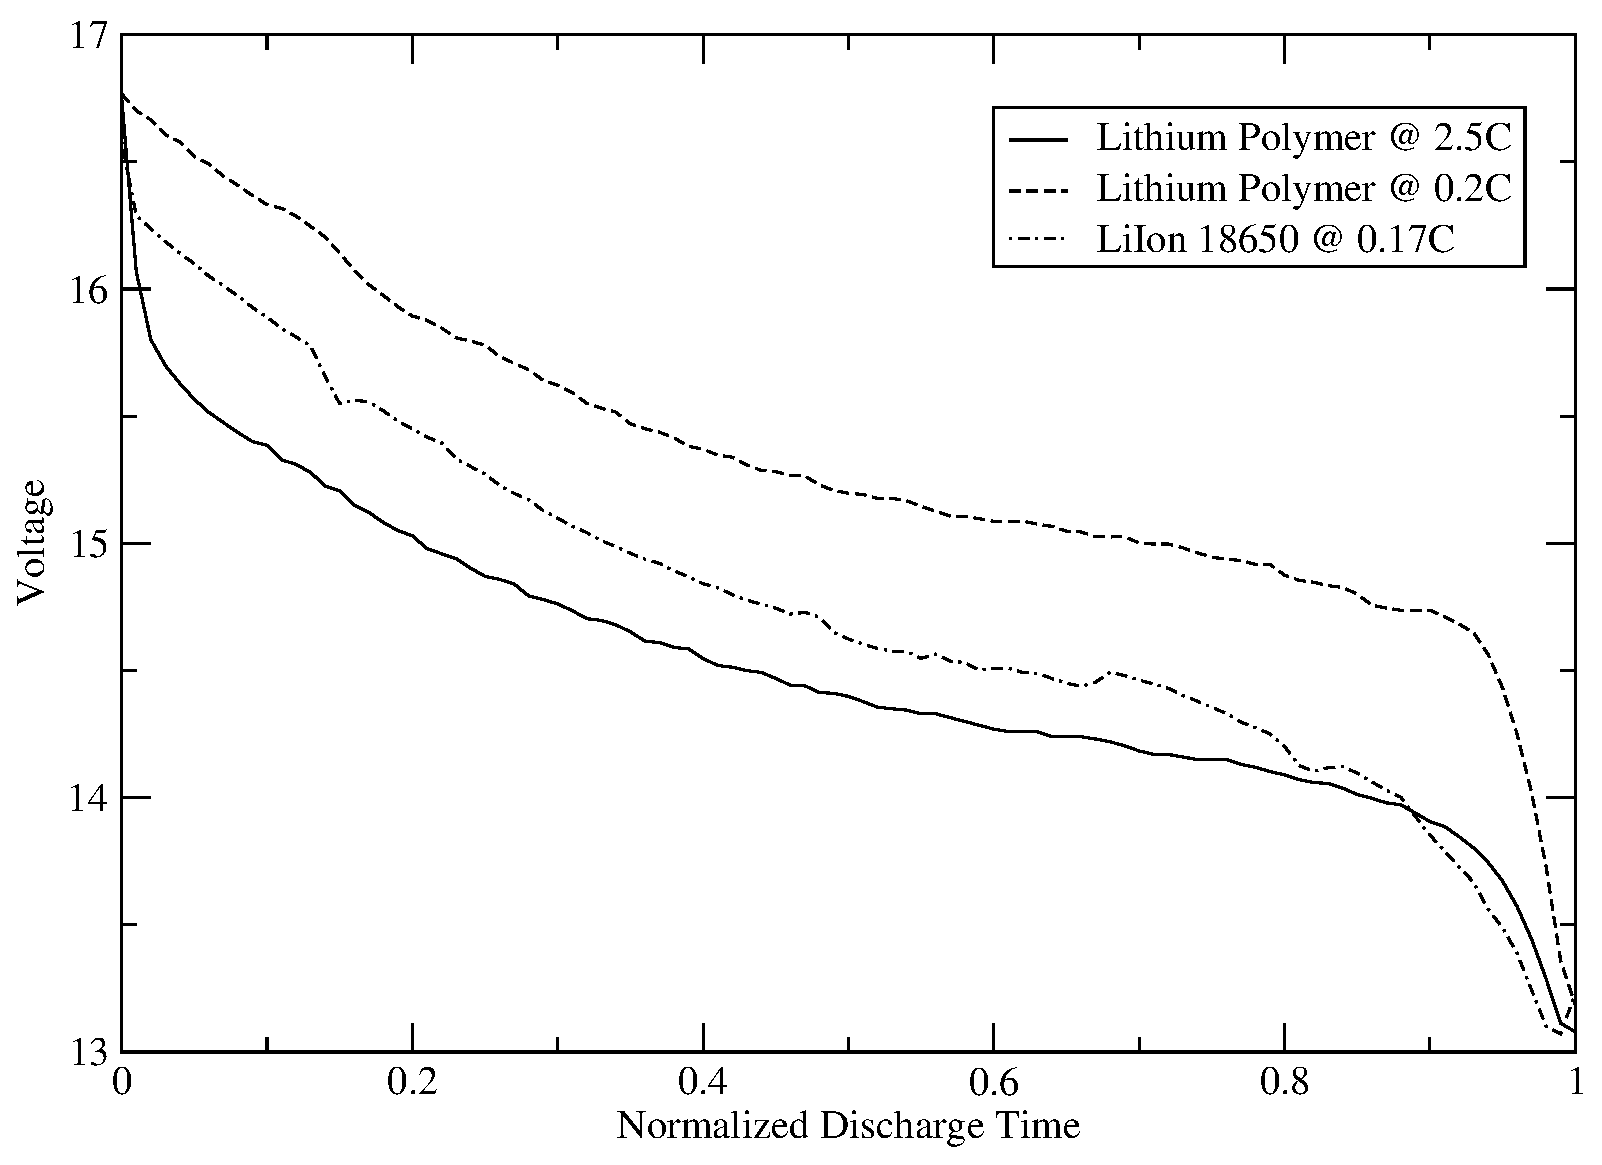
\includegraphics[width=6cm]{Figures/V_versus_T_mod.eps}
%  \caption{Pack voltage as a function of normalized discharge time for
%  2 different chemistries of the   battery packs at different discharge rates.}
%  \label{fig:Batt_v_vs_t}
%\end{figure}
%%%%%%%%%%%%%%%%%
%
%Figure \ref{fig:Batt_e_vs_t} illustrates how much energy can be extracted
%from the same sample batteries at different discharge rates. During the
%experiment, the discharge cycles were halted when the pack voltage reached
%3.2 V/cell or 12.8 V for the pack. The measured useful pack energy and
%energy-density are shown in Table~\ref{Batt_performance}.
%%%%%%%%%%%%%%%%%
%\begin{figure}[thbp]
%  \centering
%  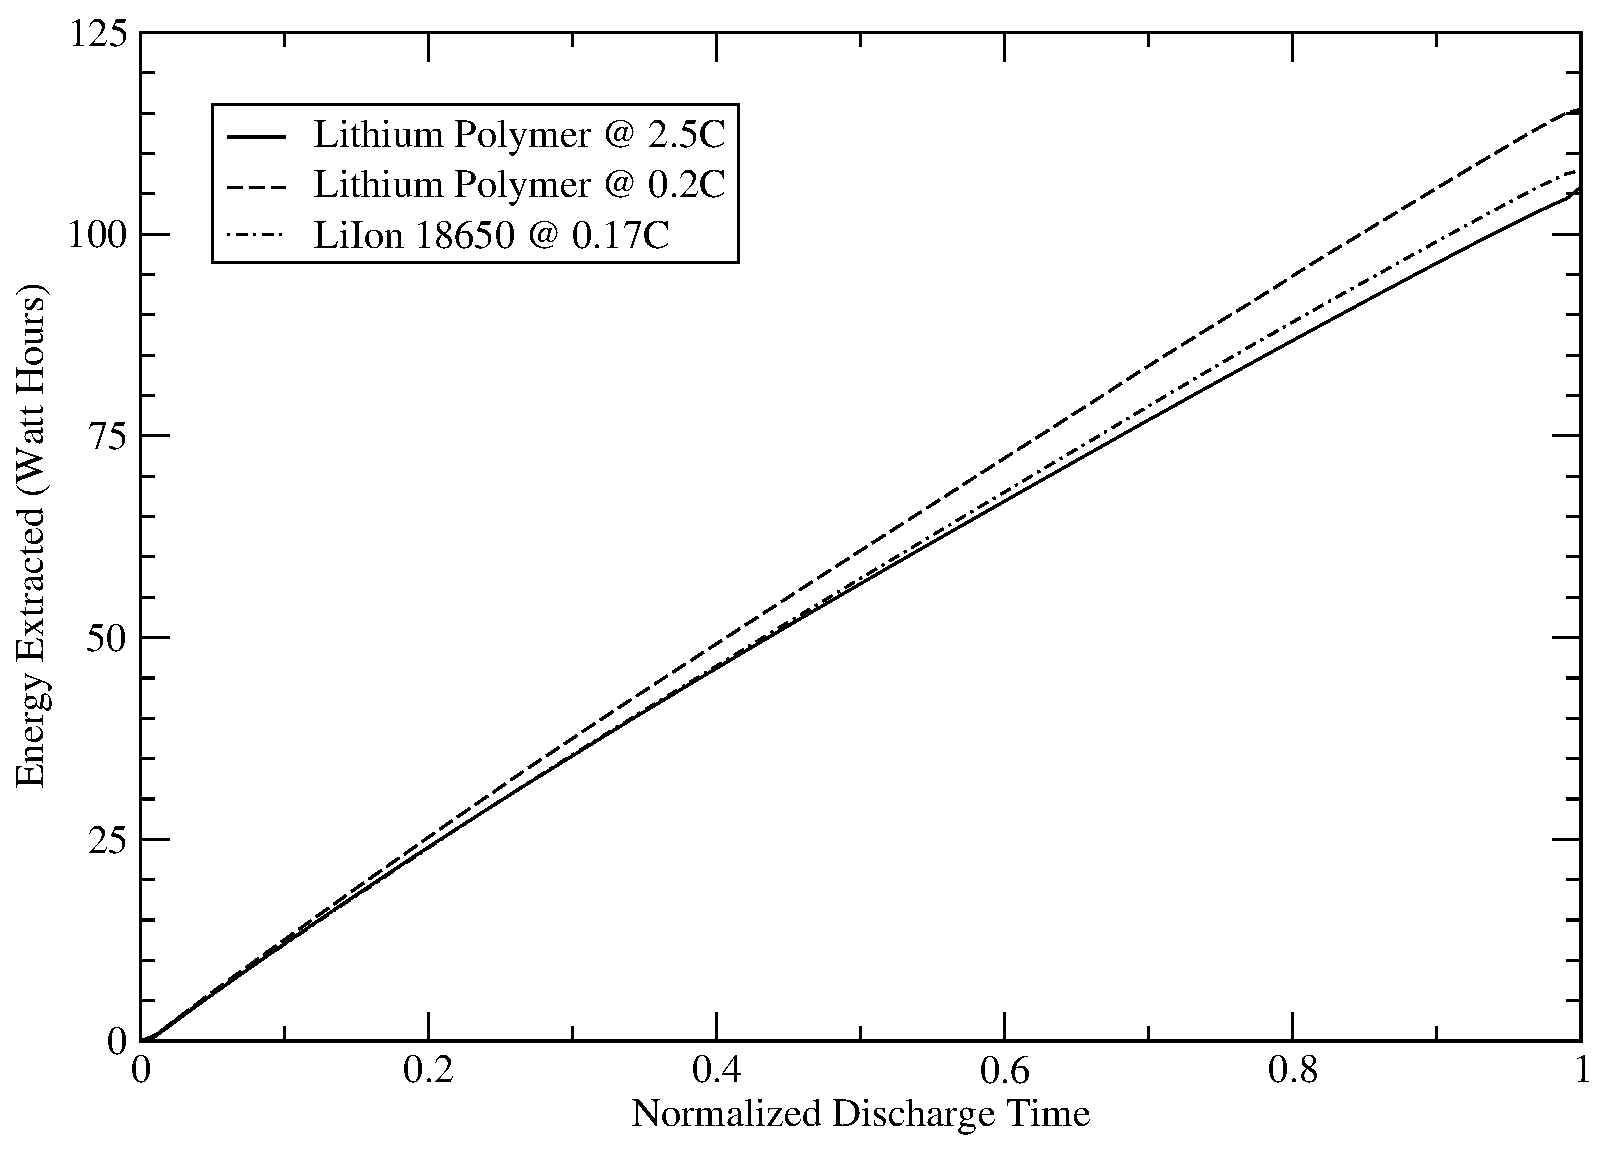
\includegraphics[width=6cm]{Figures/Energy_v_time_mod.eps}
%  \caption{Energy output as a function of normalized discharge time for
%  different discharge rates; at 1C rate the discharge current discharges
%  the battery in 1 hour.}
%  \label{fig:Batt_e_vs_t}
%\end{figure}
%%%%%%%%%%%%%%%%%
%\begin{table}
%  \caption{Measured battery performance}
%  \centering
%  \begin{tabular}{ l | r | r | r }
%  Type &C-rate & Energy (Wh) & Energy Density (Wh/kg) \\
%  \hline
%  LiPo & 0.209 & 115.5 & 177.7 \\
%  LiPo & 2.502 & 105.8 & 162.8 \\
%  LiIon & 0.171 & 107.9 & 167.3 \\
%  \end{tabular}
%  \label{Batt_performance}
%\end{table}
%%%%%%%%%%%%%%%%%
%While the sensitivity to drain rate is clear, it is also clear that
%advertised energy and energy-density might not be achievable in a practical
%application. While the LiIon cells would appear to be far superior based on
%manufacturers' specifications, experiments suggest that LiPo batteries are
%superior for onboard integration.

%A number of other uncertainties and design considerations also need to be
%identified and formalized. Among them are the structural integrity of the
%wings and the PV cells under the flex load in flight, dissipation of heat
%induced by the dark surface of solar panels and its effect on the structural
%integrity,  performance of the MPPT unit under the variable exposure of the
%PV cells to the sun, stability of the battery chemistry under variable
%temperature, losses in the mechanical gear system and the propulsion motors
%at different load, to name a few. Moreover, it is needless to say that
%PV-enhanced system may gain energy, however it won't help if the aircraft
%loses that same energy through increased viscous drag or loss of lift.
%Therefore the cells need to be built into the wing surface such that they are
%conformal with only subtle fine-texture differences.
%
%Therefore, the ultimate objective of the electrical system design is to
%obtain a representable mathematical model of the solar-powered energy
%generation, storage, and the energy expenditure system that can be identified
%on the ground and during the flight of a particular glider. The need for
%onboard identification arises as the properties of the system are expected to
%change over time; for example the batteries capacity changes with the number
%of discharge cycles.

Addressing this challenge, the project builds a prototype of the onboard
electrical system that consists of the semi-rigid research-grade mono-crystalline
Silicon cells with an advertised efficiency of 22.5$\%$, MPPT unit,
rechargeable batteries with balancing circuitry, and the load represented by
the well-defined power load of avionics and the uncertain load of the
propulsion system. An example of the laboratory prototype used for multi-day
data acquisition and system identification experiment is presented in
Fig.~\ref{fig:Solar_arch}.

%%%%%%%%%%%%%%%%
\begin{figure}[thpb]
  \centering
  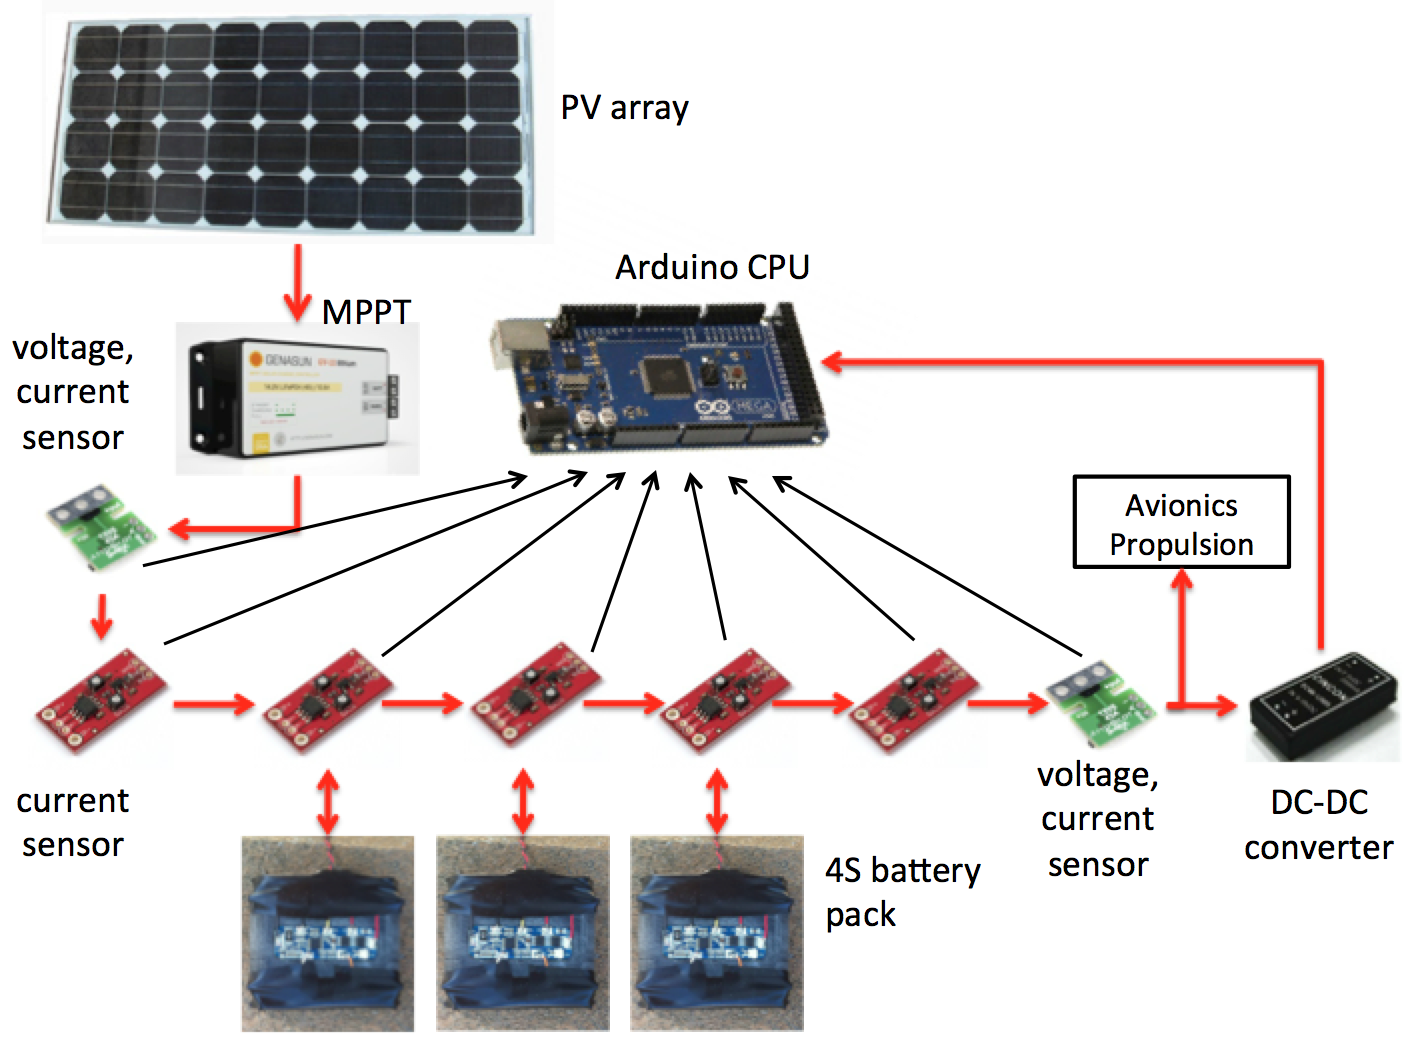
\includegraphics[scale=0.325]{Figures/Solar.eps}
  \caption{Laboratory prototype of the solar-driven electrical management system.}
  \label{fig:Solar_arch}
\end{figure}
%%%%%%%%%%%%%%%%

An example of multi-day experiment focused on formal characterization of the
system is presented next in Fig.~\ref{fig:MultiDay_enrg}. The data
illustrates the time history of electrical energy input from the PV array,
the dynamics of the batteries charge and discharge under the constant load,
and the estimated losses of energy due to the wiring, data acquisition
sensors and adverse uncertainties. Close inspection of the data suggests that
the state dynamics of batteries (both charge and discharge) can be accurately
described by the first order differential equations, while the solar input is
closely represented by the gain that is directly proportional to the angle of
incidence toward the sun.
%Although not representing all the envisioned flight
%conditions, the result still allows to recognize the key functions that can
%be used to formally describe the states of the system components and the
%total electrical energy balance.
%% it would be nice to have those functions presented here as a logical sequence%
%When the result is further enhanced with the feedback from
%the flight dynamics and the operational environment, it can be used to
%precisely characterize the range and endurance of a particular glider
%platform. The system identification phase of this work is under way.
%%%%%%%%%%%%%%%%
\begin{figure}[thpb]
  \centering
  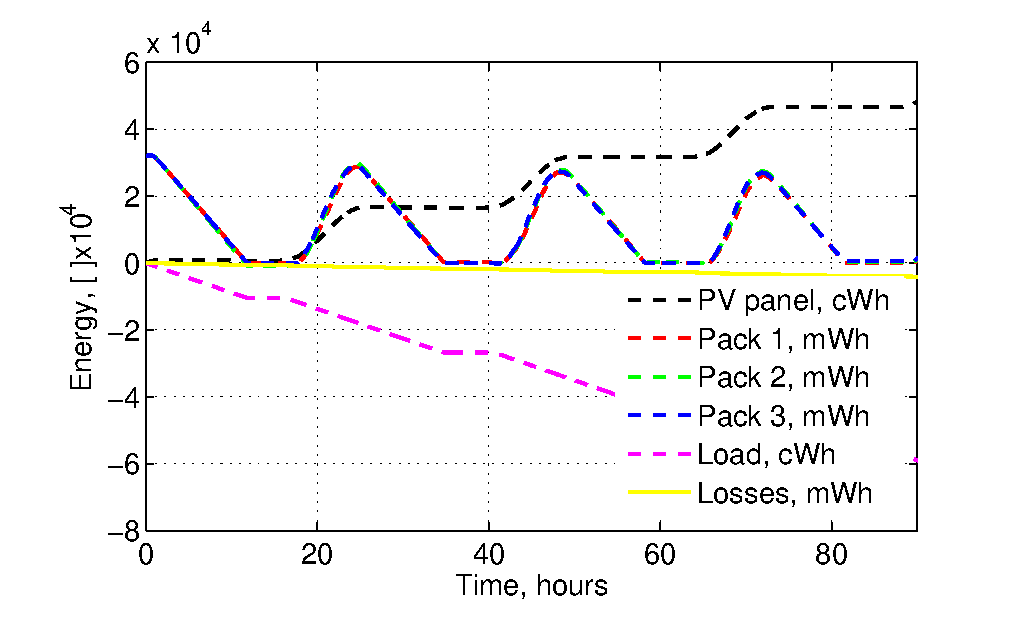
\includegraphics[scale=0.5]{Figures/MultiDay_energy_2.eps}
  \caption{Results of the multi-day experiment with the prototype
  installed in a fixed location.}
  \label{fig:MultiDay_enrg}
\end{figure}
%%%%%%%%%%%%%%%%
\squeezeup
%Earlier it was mentioned that solar radiation could be given empirically for
%a given location and time of year. This provides an estimate of what
%energy-density might be available from solar radiation. Knowing an array
%size, cell efficiency, and with estimates of air clarity, an estimate for
%available energy input from the array over a 24-hour period may be made. The
%current glider is outfitted with research-grade mono-crystalline Silicon
%cells with an advertised efficiency of 22.5$\%$.
%
%The cells are semi-rigid - they don't qualify as flexible, but they can very
%carefully be bent to conform to the airfoil surface over the majority of the
%wing. Ideally, as much of the aircraft surface as possible should be covered
%by the array, but it must be done in such a way that it does not disturb the
%boundary layer. While the system may gain energy through the array, it won't
%help if the aircraft loses that same energy through increased viscous drag or
%loss of lift. Therefore, the cells are built into the wing surface during
%initial composite lay-up of the wing, such that they are essentially
%conformal, with only subtle fine-texture differences. A small section of wing
%with embedded cells is shown in Fig.~\ref{fig:wing_sample}.
%
%\begin{figure}[thpb]
%  \centering
%  
\includegraphics[scale=1.]{Figures/IMG_3502.eps}
%  \caption{Sample wing section with conformal, embedded cells.}
%  \label{fig:wing_sample}
%\end{figure}

%In the current generation of the aircraft, a small solar array has been
%included in order to identify aerodynamic and structural issues that might
%arise. For example, the solar cells get quite hot while the aircraft is at
%rest on the ground. Will this heat be sufficient to damage the wing structure
%by softening the epoxy resin used in the composites, or delaminate the
%protective film around the cells? When the wing flexes in flight, will this
%damage the semi-rigid cells or break them loose from the wing? The current
%array includes 18 cells for an array area of 0.28 m$^2$. With the estimates
%for efficiency, this should provide on the order of 440 Wh in a 24-hour
%period in June, or roughly 50 W at mid day.
%
%Photovoltaic cells operate with variable output voltage and current which is
%dependent on the available radiation and the load impedance. In order to
%maximize power output, circuitry is required to actively adjust the load
%impedance to drive the product of voltage and current (power) to a peak. This
%device is called a Maximum Peak Power Tracker, or MPPT. The MPPT circuit uses
%switching circuitry which is typically combined with a buck or boost
%converter to yield a regulated DC voltage output. There is an efficiency
%associated with the MPPT, but it is typically quite high, typically better
%than 99 percent.
%
%The power coming from the MPPT is split and is fed into a charge controller
%for the batteries and to the load (avionics, propulsion, payload). If the
%power coming from the MPPT is greater than the load, it is used to charge the
%batteries, storing potential energy for later use. If the load is greater
%than the power coming from the MPPT then it taps into the batteries,
%depleting stored potential energy.

%Battery selection is the next challenge. Typically Lithium-chemistry
%batteries have the highest \emph{energy-density} for commercially available
%rechargeable batteries, but there is an enormous variation from type to type.
%Most suitable cell technologies fall into two categories, the \emph{can}-type
%cells usually found in laptops, and the foil-wrapped flat cells typically
%found in cell phones and other compact electronics. The can-type cells are
%usually referred to as Lithium-Ion or LiIon batteries, and the most common
%form-factor is the 18650 cell, which is nominally 18 mm in diameter and 65 mm
%long. These cells typically cannot support high discharge rates. Most are
%caped at a 1C continuous discharge rate, where the 1C rating means that the
%cell would be depleted in one hour. This equates to a low
%\emph{power-density}. This limitation will likely not be a concern, as the
%batteries are intended to be used through the night, with average discharge
%rates of less than 0.1C. Depending on the pack size, this is a potential
%limitation when the motor is used, as it is a short-term, but very high load.

%The flat foil-wrapped battery type is usually referred to as Lithium polymer
%or LiPo. These are commonly used in cell phones and other compact devices as
%well as the radio control aircraft hobby. Unlike the LiIon cells, the
%power-density of LiPo cells can be extremely high. Many in the hobby industry
%claim continuous discharge rates of 70C with bursts of up to 140C. This
%equates to draining the battery in less than one minute. Unfortunately, there
%is an inverse relationship between energy-density and power-density in these
%cells. In order to achieve the high discharge rates, the cells need more
%copper to carry the current, and the cells must be larger and heavier.

%Analyzing manufacturer specification for the LiIon cells, energy densities in
%excess of 200 Wh/kg are frequently listed, whereas for the lower
%discharge-rate LiPos the highest is on the order of 190 Wh/kg. Samples of
%both cell types were tested in current project. The LiIon cells had an
%advertised capacity of 3 Ah, and an energy density on the order of 220 Wh/kg.
%The LiPo cells had an advertised capacity of 2 Ah, and an energy density of
%just over 190 Wh/kg. Experiments were set up to test the cells under typical
%loads. Twelve LiIon cells were formed into a pack of 4 cells in series (4S)
%and 3 cells in parallel (3P), to make a 4S3P pack with a nominal voltage of
%14.8 V and capacity of 9 Ah. Sixteen LiPo cells were formed into a 4S4P pack
%with nominal 14.8 V and 8 Ah capacity.

%Due to internal cell resistance, the usable energy in the packs is a function
%of discharge rate. The LiPo pack was tested at two discharge rates, 0.21C and
%2.51C, with voltage and current logged from start to finish. The LiIon pack
%cannot support the higher discharge rate, but was tested at a lower 0.17C
%rate. Results of the discharge tests are shown in Figs.~\ref{fig:batt_v_vs_t}
%and \ref{fig:batt_e_vs_t}, plotting voltage and energy-use as functions of
%normalized discharge time, respectively. As with most batteries, voltage
%slowly drops over the discharge cycle, a feature that is convenient for
%estimating remaining energy in the pack. The voltage also drops as a function
%of load, which is a result of the internal cell resistance and Ohm's law.
%
%\begin{figure}
%  \centering
%  \includegraphics[width=82mm]{Figures/V_versus_T.eps}
%  \caption{Pack voltage as a function of normalized discharge time.}
%  \label{fig:batt_v_vs_t}
%\end{figure}
%
%\begin{figure}
%  \centering
%  \includegraphics[width=82mm]{Figures/Energy_v_time.eps}
%  \caption{Energy-out as a function of normalized discharge time.}
%  \label{fig:batt_e_vs_t}
%\end{figure}
%
%The discharge cycles were halted when the pack voltage reached 3.2 V/cell or 12.8 V for the pack.
%For the LiPo pack this is considered to be the lowest, safe voltage for the cells, The
%LiIon packs can typically be safely drained to a lower voltage, although it is apparent from
%Fig.~\ref{fig:batt_v_vs_t} that the voltage has already dropped off the cliff, and there is
%very little actual energy left in the pack. The measured useful pack energy and energy-density
%are shown in Table~\ref{batt_performance}.
%\begin{table}
%  \caption{Measured battery performance}
%  \centering
%  \begin{tabular}{ l | r | r | r }
%  Type &C-rate & Energy (Wh) & Energy Density (Wh/kg) \\
%  \hline
%  LiPo & 0.209 & 115.5 & 177.7 \\
%  LiPo & 2.502 & 105.8 & 162.8 \\
%  LiIon & 0.171 & 107.9 & 167.3 \\
%  \end{tabular}
%  \label{batt_performance}
%\end{table}
%
%The sensitivity to drain rate is clear. Also clear is the fact that advertised energy and
%energy-density might not be achievable in a practical application. While the LiIon cells would
%appear to be far superior based on manufacturers' specifications, experiments would tend to
%suggest that LiPo batteries are superior for this project.
%
%Battery capacity is driven by the need to survive the night with no photovoltaic energy input. At
%a minimum the battery must power the avionics and payload components that are in use.
%Thermal activity will diminish at night, although the same algorithm that exploits thermal lift
%during the day may be used to minimize sink during the night. If there are pockets of air
%that sink, there must be pockets of air that rise. The lift may be weak, but better than no lift
%at all. When the lift is insufficient to maintain altitude, the motor must be used to
%regain it.
%
%Use of the motor for propulsion introduces additional efficiency considerations. The motor is a
%sensorless brushless motor with electronic speed control. Motor efficiencies are quite high
%at nominal power settings. All brushless motors have internal resistance and a parameter called
%$I_0$ that represents the no-load current at a specific voltage. These two terms dictate the
%efficiency of the motor over its useful power spectrum. With no load they will draw power from
%the system that is roughly $I_0*V$ and at an efficiency of zero. As the mechanical load is
%increased, the efficiency rapidly increases to some peak value. While the motor might have a
%nominal efficiency of better than 90 percent at its rated power, at a much lower power the
%efficiency can be very low, perhaps below 50 percent. This becomes critical when the motor is
%used for propulsion. The current airframe at nominal weight requires on the order of 40 $W$ to
%sustain cruise flight, but the motor is rated for up to 1000 $W$. At full throttle with the
%included gear drive and propeller it draws on the order of 400 $W$ with an estimated total
%efficiency in excess of 85 percent, but at 40 $W$ the system efficiency is down around 10
%percent. This is a clear indication that when the motor is used, it should be used at a high
%power
%setting, not to sustain cruise flight, but to actively gain altitude, using elevation as energy
%storage. The intermittent high power draw from the propulsion will reduce the battery
%efficiency somewhat, but this is much more subtle than the motor efficiency curve.

\subsection{Glider Identification and Updraft Detection}
\label{subsec:SysID}
\squeezeup
There is a number of prior efforts devoted to the thermal soaring flight.
First demonstrated by human pilots in 1900s (see \cite{Simons:1998}) the idea
of soaring in convective air became feasible for onboard autonomous
implementation only in the 1990s, see \cite{Wharington:1998}. While enabling
the desired functionality by primarily mimicking the birds flight and indeed
achieving significant extended flight capabilities (see \cite{Edwards:2008},
\cite{Allen:2006}, and \cite{Allen:2007}), most of the algorithms used
heuristics in finding an updraft and the identification of its strength, its
potential utility in energy gain, and the decision of how to stay in the
updraft. The reason for employing heuristic approaches is obvious, since both
the strength of the updraft and its efficiency are both subject to
significant uncertainties and are hard to formalize.
%First, they result from the uncertain flight characteristics of the specific glider no
%matter how well the airframe is modeled and flight tested. ; significant advances in
%material and structures sciences produce novel airframes that are strong and flexible on
%one hand, and therefore aerodynamically uncertain when bend and twisted on the other
%hand.
%Next, when a glider moves through unsteady air the estimation of the updraft
%strength and geometry, which are critical utility parameters of the updraft,
%significantly lacks of spatial content in noisy onboard measurements. Thus,
%it takes significant time before the updraft utility is identified and the
%guidance algorithm is engaged.
The heuristic nature and the noise in measurements lead to significant time before the updraft  is identified and the guidance algorithm is engaged.

%
%It is worth noting, that when controlled by the thermal centering guidance law the
%estimation algorithm partially regains the spatial data in horizontal direction.
%
%The approach used in our development shifts the focus from heuristics toward
%the online estimation of the glider flight dynamics and the parameterized
%model of the convective updraft.

To formalize the detection of thermals we develop an algorithm that is based on two complementary approaches. The first approach utilizes the inherent sink rate polar, and the
second one is based on the total energy of the system. Conceptually
they are similar as they compare the natural metrics of the system with the
same metrics measured in flight.

%Moreover, as an effective method of rapid identification of $3D$ energy
%profile of a thermal updraft, we utilize multiple collaborative platforms
%that simultaneously sample the same updraft in $3D$ and share the
%spatially-rich data to speedup the estimation process.



%\emph{The sink rate polar} is the curve of the vertical speed plotted versus the true air
%speed (TAS). Every glider has a very specific sink polar as it reflects the glider
%inherent ability to descend in wings level flight in no-wind conditions; sink polar can
%be obtained to characterize the sink rate at various bank angles that can be used to
%minimize the energy loss in turning flight. Thus, if the sink polar is known then the
%difference between the actually measured sink rate and the point on the sink polar
%corresponding to the measured true air speed identifies if there is an excess of energy
%in the air that forces the glider away from its native sink polar; the sign of the
%difference defines the updraft and downdraft conditions. Implementation of this approach
%depends on precise characterization of the sink polar of the glider that can be
%practically achieved in extensive experimentation. However, experimentation can hardly
%provide an ideal controlled conditions, and in every flight of the same platform there
%are always subtle differences that are not accounted for. Based on the extensive
%experimental data collected an a number of flights (see \cite{AKlass_JGCD:2012} and the
%references herein) in close to ideal no-wind conditions the sink polar was first obtained
%off-line. Analysis of the measurements confirmed that the sink polar can be represented
%by a second order polynomial $V_s=A \cdot V_{tas}^2 + B \cdot V_{tas} +C$ with
%coefficients $A, B$, and $C$ defined by the least squares approximation method; similar
%results can be found in \cite{Reichmann:1978}, \cite{Edwards:2008}. The same method is
%then implemented onboard as a recursive least square (RLS) estimator, see
%\cite{Astrom:1995}, to account for any variations in the setup of the actual flying
%platform. A comparative example of identifying the sink polar of ASW-27 glider using the
%developed algorithm and the experimentally verified data  from \cite{Boermans:1994} is
%presented in Fig.~\ref{fig:SinkPolar}. The identification algorithm was tested against
%the flight data  of ASW-27 acquired in high-fidelity simulation provided by the Condor
%software (\cite{Condor:2013:Online}), see details in Section.\ref{sec:SimEnv}.

\emph{Characterization of the sink polar} - the function of vertical sink
rate versus the true airspeed (TAS) - of a particular glider can be
practically achieved in extensive experimentation. However,
flight-experimentation in real-world environment can hardly provide ideally
controlled conditions. In the developed approach, the estimates of the
sink-polar were first made by post-processing a collection of experimental
flight results obtained in low-wind, low-lift conditions, see
\cite{AKlass_JGCD:2012}. Sink polars are roughly quadratic in nature, thus a
least-squares approach yields suitable coefficients based on the historical
data. Further in flight, a recursive linear least square estimator is used in
real-time to account for specific variation in the platform and atmospheric
conditions at that moment. An example of accuracy of this approach is
presented below in Fig.~\ref{fig:SinkPolar} for a full-scale ASW-27 glider;
the result was obtained using the Condor simulator
(\cite{Condor:2013:Online}) and ''true`` data of \cite{Boermans:1994}, see
more details in sec.\ref{sec:SimEnv}. The detection of a thermal and
estimation of its intensity, that contributes to the recursive identification
of its parameters (see sec.\ref{subsec:BayesianMapping}), are based on
comparison of the currently measured sink rate with the sink rate predicted
by the polar for a measured TAS; if the measured sink rate is smaller than
predicted, then there is a thermal.
%%%%%%%%%%%%%%%%
\begin{figure}[thpb]
  \centering
  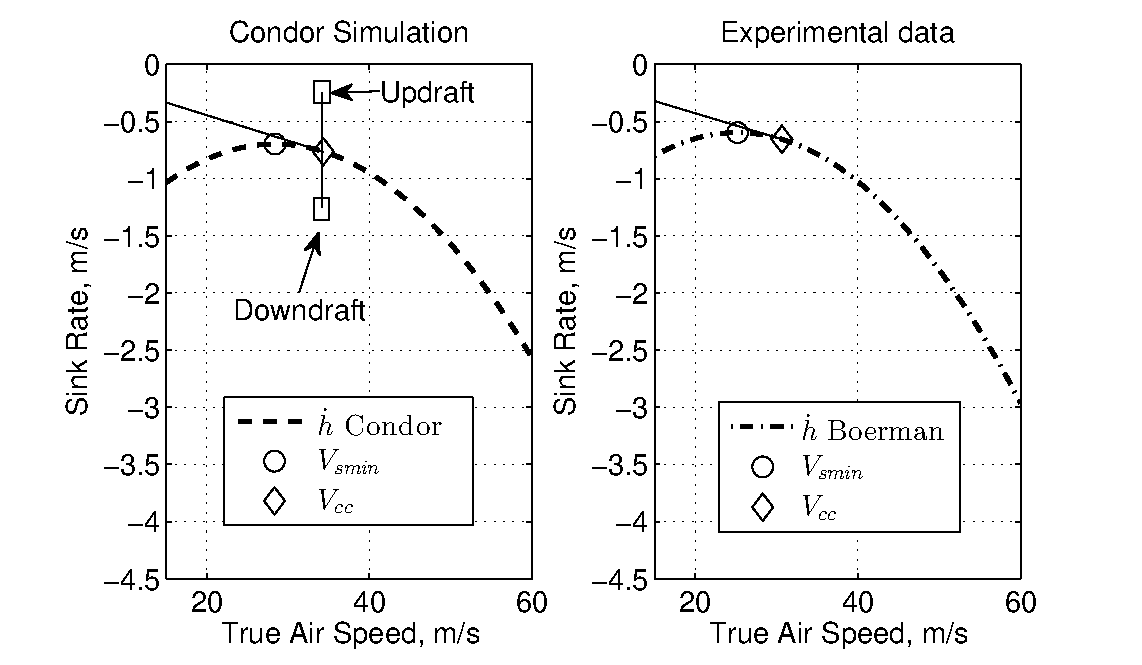
\includegraphics[scale=0.48]{Figures/Condor_Boermans_comparison_mod_2.eps}
  \caption{The identification of the inherent sink rate polar.}
  \label{fig:SinkPolar}
\end{figure}
%%%%%%%%\cite{Piggott:1997} and%%%%%%%%
The analytical representation of the sink rate polar contributes not only to the
identification of thermal updrafts, but also to the mission planning of a
specific glider, see ~\cite{FAA:2011}. In particular,
the polar defines the minimum sink rate $V_{s}min$ and the corresponding TAS
command for the autopilot to follow. While $V_{s}min$ may be too close to the
stall speed $V_{stall} \approx V_{s}min$ and should be avoided, the effective
speed commanded in thermaling mode $V_{th}$ may be higher. The polar
also defines the optimal TAS command $V_{cc}$ for the maximum glide ratio
flight that is used by the navigation task in planning for the maximum range
''cross-country`` segment; the tangent line from the origin defines $V_{cc}$.
%While the sink polar should be ideally obtained in no-wind environment, its
%application to the known wind conditions is also straightforward and allows
%for the calculation of the distances to be traveled in cross-country flight,
%see more details in \cite{Piggott:1997} and \cite{FAA:2011}.

\emph{The total energy} approach is also widely used in human piloted soaring
flight. It is based on the concept that the mechanical energy $E_{tot}$ of
the soaring glider combines the potential energy, $E_p=mgh$, and kinetic
energy, $E_k=\frac{m\cdot V^2}{2}$, of the airframe minus the ''leakage`` of
the energy due to the work of the parasitic and induced aerodynamic drag,
$E_{D}$. For an ''aerodynamically clean`` glider the parasitic drag is relatively
constant  with $\dot{E}_{D}\approx0$.
%with an objective to
%minimize the total energy loss, the control commands of its autopilot will
%necessarily result in mild variations of the angle of attack, thus leading to
Consequently, for the total energy and its rate of change over sufficiently
long time intervals one can consider the following:
%Therefore, for efficient airframes the value of total energy remains nearly constant over
%long periods of time with its rate of change close to zero, $\dot{E}_{tot}\approx0$, if
%there is no propulsion or external energy injected. To be more precise, it is
%''slightly`` negative, $\dot{E}_{tot}<0$, thus, in fact, being the only reason for a
%glider to descent naturally.
\begin{eqnarray}
    && E_{tot}=mgh+\frac{m\cdot V^2}{2}-E_{D}, \quad E=\frac{E_{tot}}{mg}, \nonumber \\
    && \dot{E}=\dot{h}+\frac{V \cdot \dot{V}}{g}, \quad \ddot{E}=\frac{\dot{V}^2 + V \cdot
    \ddot{V}}{g} + \ddot{h},
    \label{eq:totenergyrate}
\end{eqnarray}
where $m$ is the mass of the airframe, $g$ is the gravitational constant, $E$
is the normalized total mechanical energy of the system (also called the
specific energy), $h$ is the height, and $V$ is the inertial speed.
Therefore, the longitudinal long period oscillations represent the natural
tradeoff of kinetic and potential energy while their sum remains nearly
constant. As a consequence, in no updraft conditions the rate of change of
the total energy $\dot{E}\approx 0$. Therefore, if there is a significant
variation of the total energy, then the energy rate will be significantly
away from zero thus indicating the energy variation due to vertical airflow.
In fact, the total energy management just presented is widely used in manned
aviation being implemented in the so-called total energy compensating (TEK)
variometer, see for example \cite{PitLab:2013:Online}.

All the components of equation (\ref{eq:totenergyrate}) are available in
onboard autopilot. Both equations in (\ref{eq:totenergyrate}) are included
into one Kalman filter along with the inertial and barometric sensors
outputs. The resulting energy rate-based solution provides another accurate
indication of the updraft event. A comparison of the output of the total
energy approach with the output of the TEK variometer $\dot{h}_{TEK}$ is
presented next in Fig.~\ref{fig:ThermalDetection}.
%%%%%%%%%%%%%%%%
\begin{figure}[thpb]
  \centering
  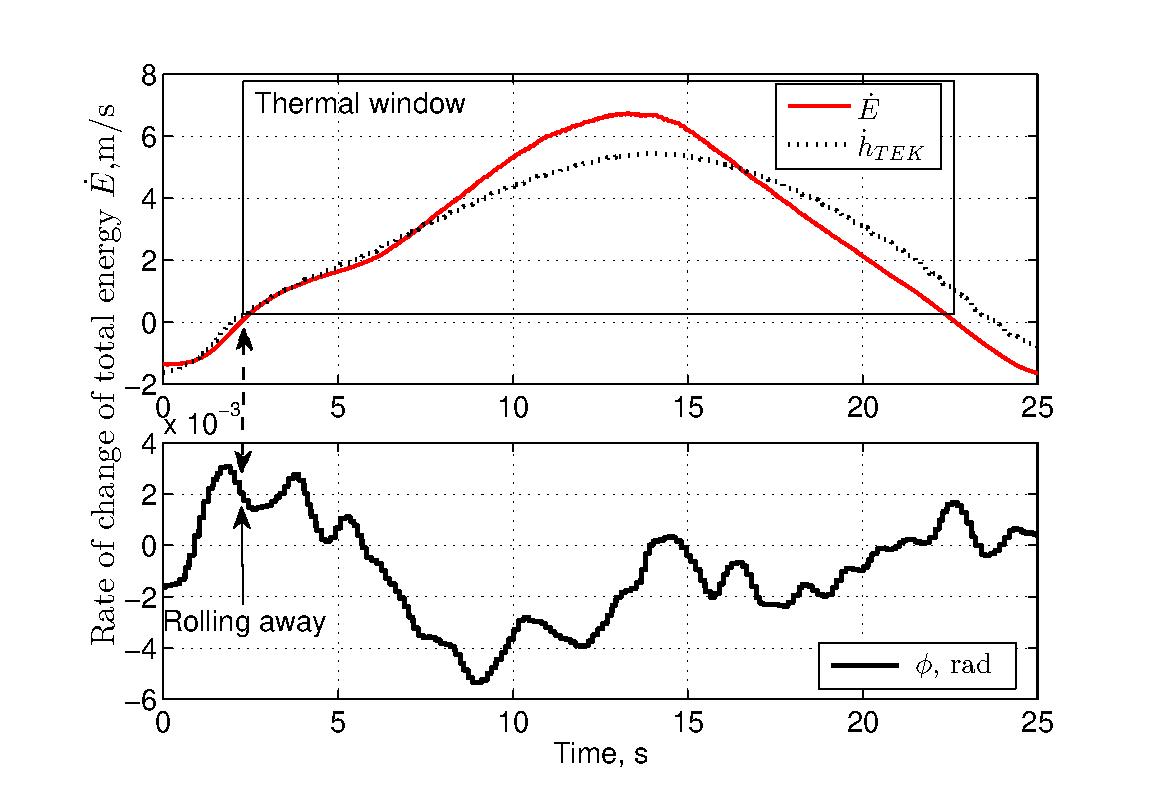
\includegraphics[scale=0.44]{Figures/TEK_Bank_2.eps}
  \caption{Energy-based detection of updrafts; the data is simulated
  by the~\cite{Condor:2013:Online} software, see sec.\ref{sec:SimEnv}.}
  \label{fig:ThermalDetection}
\end{figure}
%%%%%%%%%%%%%%%%
\squeezeup
%The outcomes of the total energy estimator in (\ref{eq:totenergyrate}) are used in the guidance
%law implementation that is presented next.

\subsection{Guidance in Thermal Centering Mode}
\label{subsec:ThermGuidance}
\squeezeup
When a thermal updraft is detected the glider needs to automatically maneuver
to enable staying in the thermal with the objective of increasing the
glider's potential energy through a rapid increase of the height. The
theoretical development of the thermaling guidance law has been recently
reported in \cite{AKlass_JGCD:2012}). The most recent experimental results
and findings that motivate further refinement of the solution were discussed
in \cite{AKlass_CDC:2012}. This development was recently modified to include
the sign of the turn rate command that is defined by the estimate of the body
roll angle $\phi$; it was observed in a number of flights that entering the
thermal induces the motion that rolls the wings away from the thermal (see
Fig.~\ref{fig:ThermalDetection}), thus suggesting the turn in opposite
direction.
%The resulting thermaling guidance law implemented onboard
%of real glider enabled successful latching and effective exploitation of the
%thermal.

The thermal centering guidance law produces a turn rate command
$\dot{\psi}_{c}$ to the autopilot, and is based on the feedback control law
that takes into account the desire to get closer to the updraft center
(defined by the $\rho_d$), where its intensity (the positive vertical speed)
is the highest. On the other hand, the control balances the height increase
and the turn-induced sink rate by a measure proportional to the rate of
increase of the total energy (defined by the $\ddot{E}$ in
(\ref{eq:totenergyrate})), see the geometry of the guidance task in
Fig.~\ref{fig:ThermaG} and the resulting guidance law in
(\ref{eq:GuidanceLaw}):
\begin{eqnarray}
    && \dot{\psi}_{c}=\frac{V}{\rho_d}-k_1 \cdot \ddot{E},
    \label{eq:GuidanceLaw}
\end{eqnarray}
where $\rho$ and $\rho_d$ are the current distance and the desired orbital
radius around the center of the thermal updraft, and $k_1$ is the feedback
gain determined by the stability and performance requirements.
\begin{figure}[thpb]
  \centering
  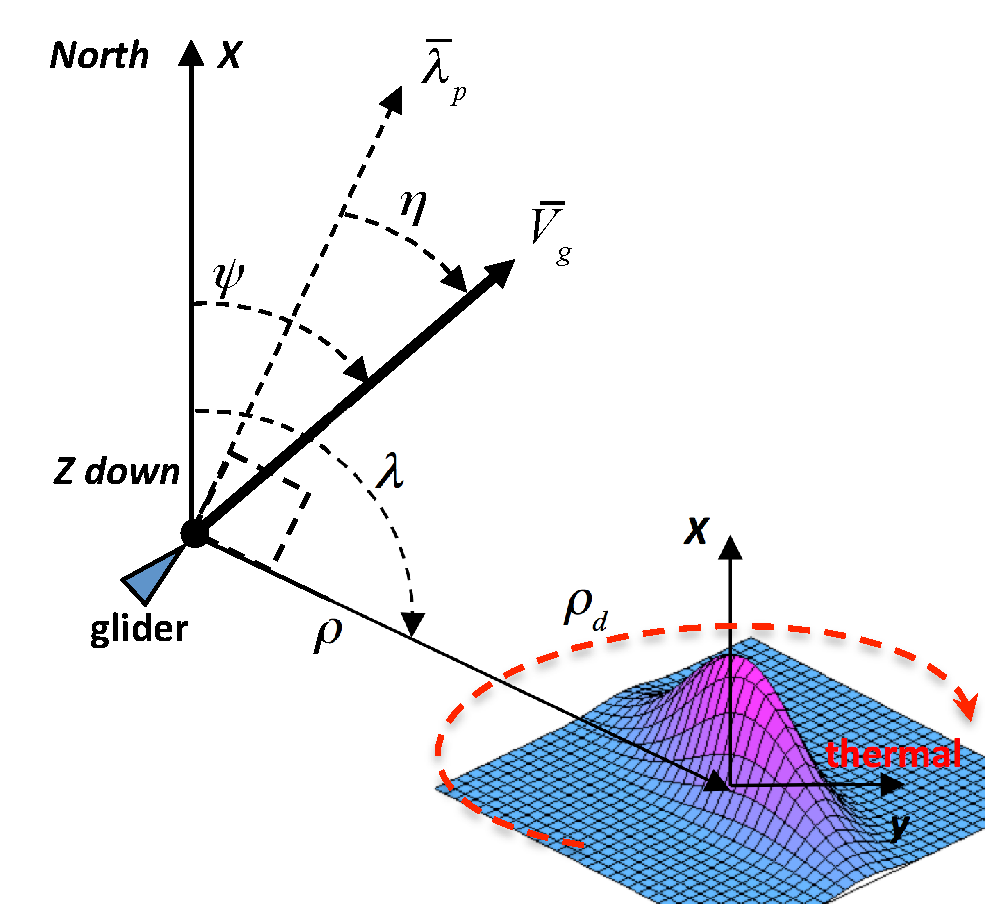
\includegraphics[scale=0.3]{Figures/ThermalG.eps}
  \caption{Kinematics of guidance around a stationary thermal updraft.}
  \label{fig:ThermaG}
\end{figure}
For the feasibility of theoretical development the thermal center is assumed
stationary with its position unknown. The desired distance ($\rho_d$) toward
the center at this point is not defined, however for the stability of the
control law it is assumed to be away from zero. The best value of $\rho_d$ is
initially assigned based on statistical observations of the glider
performance and the shapes of updrafts in the area. Later on, when
collaborative gliders contribute to the identification of the updraft
geometry this value is updated, thus resulting in a feedback that improves
the collaborative efficiency of utilizing the free energy of the updraft. For
the stability analysis of the thermaling guidance law it is assumed that the
intensity of the updraft can be represented by the Gaussian distribution
function of the form:
\begin{eqnarray}
    && \omega=\omega_p \cdot e^{-[\frac{(x-x_0)^2+(y-y_0)^2}{2\sigma^2}]},
    \label{eq:GaussUpdraft}
\end{eqnarray}
where $x, y$ represent the coordinates of the glider, $x_0, y_o$ represent
the unknown coordinates of the center of updraft, $\omega_p$ is the peak
intensity of the updraft,and $\sigma$ defines the geometry of the symmetric
updraft (in general case $\sigma_x \neq \sigma_y$). For a stationary updraft
modeled by Gaussian distribution function with $\sigma>0,~\omega_p>0$ and the
glider with $V>0, \rho_d>0$, it is proven that the feedback guidance law in
(\ref{eq:GuidanceLaw}) is locally asymptotically stable with an equilibrium
at $(\eta, \rho-\rho_d)=(0,0)$ and a region of attraction $\Omega=\{(\eta,
\rho-\rho_d): \vert \rho-\rho_d \vert \leq \beta,  \vert \eta \vert \leq
\alpha \}, $ where $\beta < \rho_d, \alpha< \pi/2$, for any
\begin{eqnarray}
    && k_1 > \tan \alpha \frac{\sigma^2}{\omega_p(\rho_d-\beta)^2}
    e^(\frac{-(\rho_d+\beta)^2}{2\sigma^2} ).\nonumber
    \label{eq:GuidanceGain}
\end{eqnarray}

The physical meaning of the guidance law (\ref{eq:GuidanceLaw}) is to
increase the commanded turn rate until the rate of climb in the latched
updraft is compensated by the sink resulted from the steep banking; most
traditional autopilots implement bank-to-turn control laws.
%%%%%% need to illustrate (place a figure) how the sink polar
%%%%%% shifts down with an increase of a bank angle %%
%In fact, the sink polar diagram (Fig.~\ref{fig:SinkPolar}) and the discussion
% come handy here as they show that the sink rate gradually increases with
% the bank angle of the glider.

%\subsection{Identification of the Updraft Geometry}
%\label{subsec:UpdraftID}
%\squeezeup
%
%As described above, the thermal intensity model adopted for the stability analysis of the
%thermal centering guidance law is the 2-dimensional Gaussian distribution
%(\ref{eq:GaussUpdraft}). Although its effective application was successfully
%demonstrated, it is realized, that the thermals geometry and their motion is more
%complex: it does not only move but also bends, see \cite{Reichmann:1978} and the
%experimental result in  Fig.~\ref{fig:ThermaShape} obtained by a single glider
%persistently staying in an updraft, see \cite{AKlass_JGCD:2012}.  It can be argued
%whether Gaussian function is a good representation of a thermal or not. However, even if
%a Gaussian distribution does not encompass all the features of an actual updraft, most
%sources agree that it does capture many of the key characteristics of a real thermal,
%i.e., being strongest at the core, with a rounded shape and gradual decrease in strength
%towards the edges; see, for example, \cite{Wharington:1998} and \cite{Pagen:1992}. At the
%end, the ultimate goal of the updraft identification is to develop a georeferenced map of
%thermals in the operational area to enable intelligent mission planning with an account
%of free energy resources.
%
%%%%%%%%%%%
%\begin{figure}[thpb]
%  \centering
%  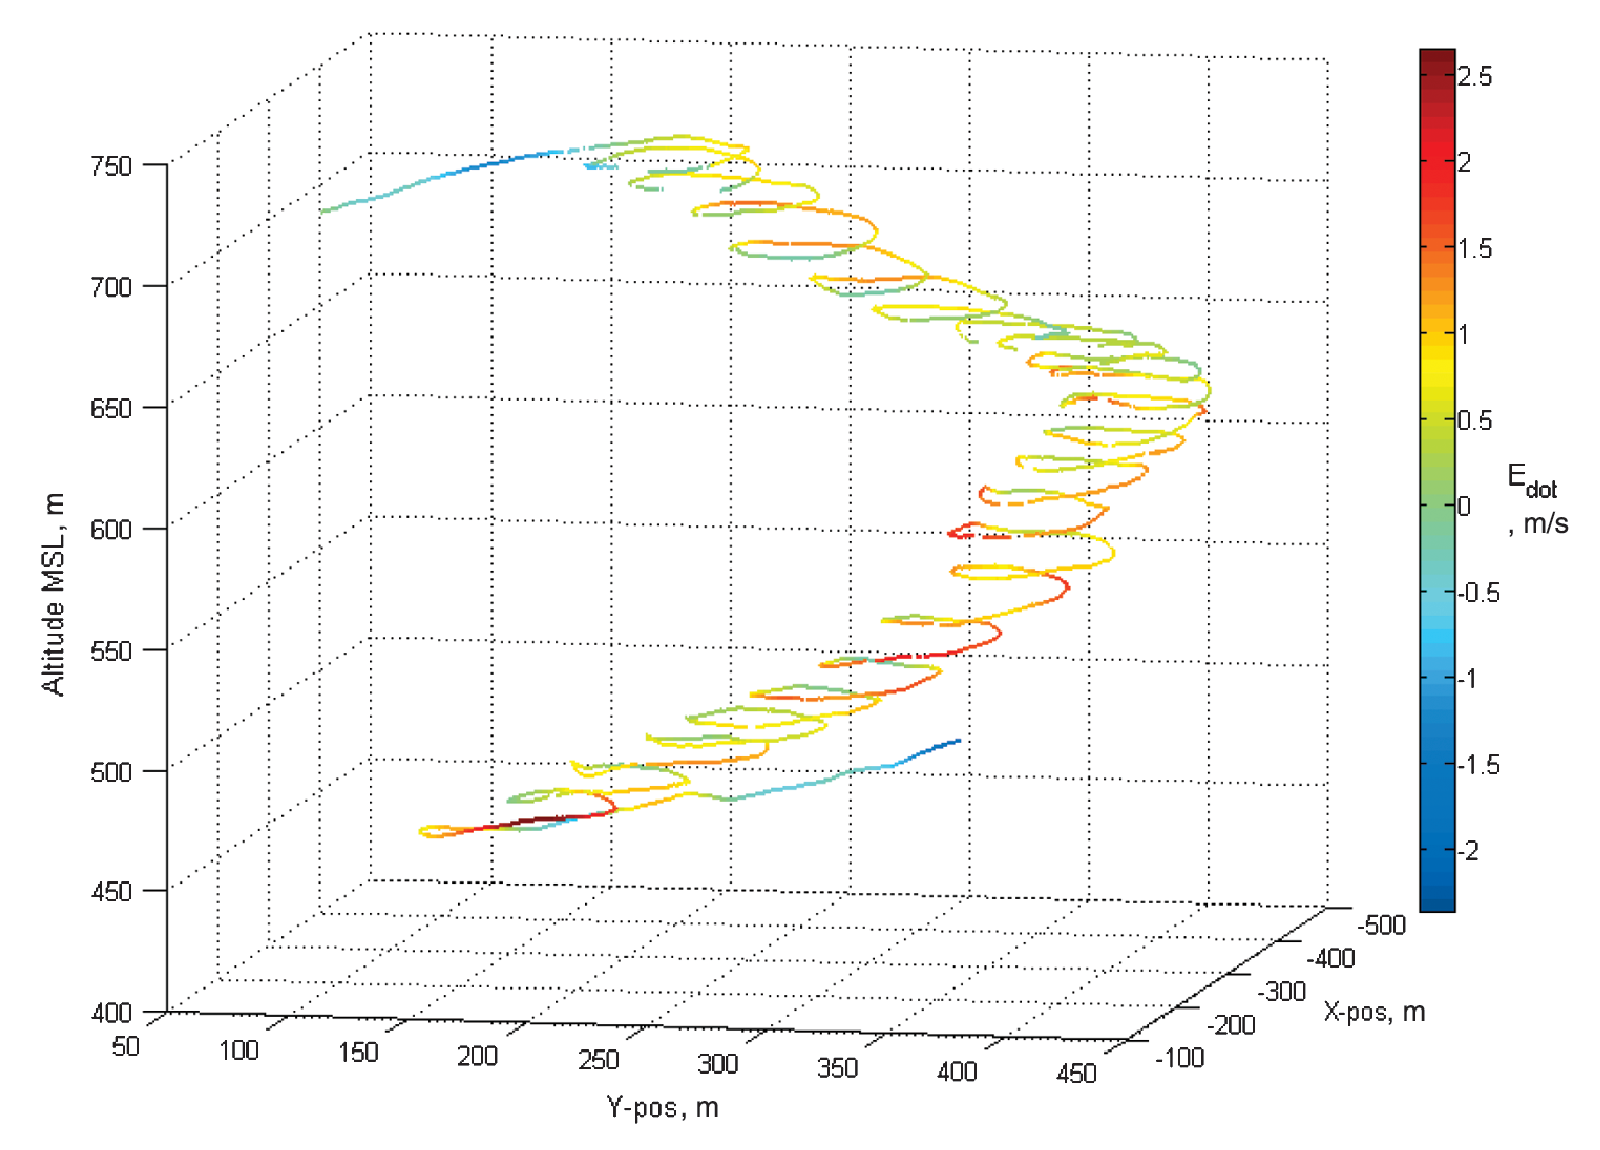
\includegraphics[scale=0.3]{Figures/BendedThermal.eps}
%  \caption{The experimentally obtained shape illustrates complex geometry of an updraft; color
%coding represents the rate of change of the total energy (\ref{eq:totenergyrate}) of a glider guided
%by  the control law in (\ref{eq:GuidanceLaw}).}
%  \label{fig:ThermaShape}
%\end{figure}
%%%%%%%%%%%

\section{Cooperative Thermals Identification }
\label{sec:CoopAlgs}
\squeezeup
The initial approach to the estimation of thermals ($2D$ coordinates of the
center vs. the glider altitude) by utilizing the measurements of single
glider in soaring mode was based on two classical nonlinear filtering
techniques: first - the nonlinear Kalman filter with the ''bearings only
measurements``, and second - the kinematic relation $\dot{\rho}=-V_g\cdot
sin(\eta)$ between the speed over ground $V_g$ and the ''navigation error``
$\eta$, see Fig.~\ref{fig:ThermaG}. In both formulations the bearing to the
updraft center was assumed to be constant at $\pi/2$ ($\lambda-\psi=\pi/2$)
with respect to the direction of turning flight; the turn is defined toward
the center of the updraft. When entering a strong updraft, the performance of
either filter was slow but reasonable, resulting in a converging solution in
about 2 full orbits and precision of the thermal center estimation of
$~75m$.
%the experimental setup unfortunately does not allow for true data of the
%thermal, while the simulation data is not a representative metric for the comparison.
%
%Although this solution might be sufficient as an initial guess for the cooperative
%navigation of multiple gliders, the design of the filter does not naturally allow for an
%effective fusion of measurements provided by multiple data-sharing gliders at different
%altitudes; even two gliders in the same thermal at different altitudes would require
%serious modification of either of the filters.

\subsection{Bayesian Identification of Thermals}
\label{subsec:BayesianMapping}
\squeezeup

To improve the efficiency of updraft estimation the solution should integrate
the knowledge gained by multiple gliders and the prior meteorological
observations (see \cite{Pennycuick:1998}, \cite{Hindman:2007}), which might
be available for the area of operation. The latter data can be conveniently
interpreted as a probability density map of convective air activity with
respect to the geographic position, see a conceptual example in
Fig.~\ref{fig:HeatMap}.
%%%%%%%%%%
\begin{figure}[thpb]
  \centering
  \includegraphics[scale=0.3]{Figures/ProbabilityThermal.eps}
  \caption{Probability map of convective air activity.}
  \label{fig:HeatMap}
\end{figure}
%%%%%%%%%%
As a first step toward cooperative identification and exploitation of
convective thermals with an account of prior methodological observation, the
probabilistic recursive Bayesian approach was adopted, see more details in
\cite{Bergman:1999} with the key ideas outlined next.

Consider a task where $N$ gliders cooperatively estimate the velocity
$f_k=f(x_k,y_k,z_k)$ of flow field at the inertial coordinates $x_k,y_k,z_k$
of $k$-th glider, $k=1...N$. Assume that the onboard instrumentation enables
measuring the lateral and vertical components of the airflow. The convective
airflow of interest is captured by a given parametric model with unknown
characteristics; see, for example, the vertical updraft model in
(\ref{eq:GaussUpdraft}) with unknown parameters $\omega_p$, $\sigma$, $x_0$,
$y_0$. The objective of the task is to estimate $f$ by using noisy
observations of the airflow provided cooperatively.

Let $X(t)=(\omega_p, \sigma, x_0, y_0)$ be a state vector that encapsulates
the unknown constant parameters of the convective flow velocity $f_k$ that is
estimated at each point of the discretized space at discrete time instance
$t$, $s_k(t)$ denote the noisy measurement of vehicle $k$ at time $t$, and
$S_k(t)=\{s_k(0),...,s_k(t)\}$ define the set of samples up to the current
time $t$. Assume that $s_k(t)$ of each vehicle at location $x_k,y_k,z_k$ is
corrupted by Gaussian noise such that
$s_k(t)=f_k(x_k,y_k,z_k)+\mu_{h,k}+\mu_{v,k}$, with $\mu_{h,k}\sim
N(0,\sigma^2_h)$ and $\mu_{v,k}\sim N(0,\sigma^2_v)$ being white noise
components in the horizontal and vertical directions.

Then in discrete settings where $t-1$ refers to the previous time step, the
conditional probability of the state $X(t)$ given the set of measurements
$S_k(t)$ of $k$-th glider alone is
\begin{eqnarray}
    && p(X(t)\vert S_k(t))=\beta \cdot p(s_k(t) \vert X)\cdot p(X(t) \vert S_k(t-1)),
    \label{eq:BayesProb}
\end{eqnarray}
where $\beta$ is the normalization coefficient chosen to guarantee that
$p(X(t)\vert S_k(t))$ at every instance of $t$ has a unity integral over the
state-space $X$.  The $p(s_k(t) \vert X)$ is the likelihood function
represented by the conditional probability of the measurement $s_k(t)$ given
the state $X$, and the $p(X(t) \vert S_k(t-1)$ is the prior probability
distribution that represents any given knowledge or intelligence about the
most likely location and intensity of thermals. In our development $p(X(0)
\vert S_k(0)$ is what encapsulates the probability ''heat map`` at the very
first step, see Fig.~\ref{fig:HeatMap}.

Finally, let each point of state $X$ be represented by the
multi-variate Gaussian likelihood function:
\begin{eqnarray*}
    && p(s_k(t)\vert X)=\frac{1}{[2\pi \Delta]^\frac{1}{2}}  exp( \frac{-[f_k(X)-s_k(t)]}{2 \sum
    [f_k(X)-s_k(t)] }),
    \label{eq:BayesLikeLH}
\end{eqnarray*}
where $\Delta=diag(\mu^2_h,\mu^2_v)$. Assuming that measurements are
synchronously taken at each time step and the gliders share the
data, the conditional probability density of the state $X(t)$ is updated
through the natural motion of the fleet of gliders sampling the airflow as
%at ($x_k,y_k,z_k$) as
\begin{eqnarray}
    && p(X(t)\vert S(t))=\beta \cdot \prod_{k=1}^N p(s_k(t) \vert X)\cdot p(X(t) \vert S(t-1)),
    \label{eq:PostProb}
\end{eqnarray}
where $S(t-1)$includes the measurements from all $N$ gliders in the fleet.
Now it is clear that the points of the parameter space corresponding to the
maximum of the posterior probability density $X(t)=\max p(X(t) \vert S(t))$
provide the maximum likelihood of the convective flow field parameters.
%
%In a verification scenario when ''true thermals`` are distributed according to the known
%''heat map`` and the prior is initialized uniformly, the recursive algorithm in
%(\ref{eq:BayesProb}) should converges   to the ''true heat map'' asymptotically.

An example of the recursive algorithm (\ref{eq:PostProb}) for the case of
three simulated gliders cooperatively flying and estimating parameters of a
single stationary updraft in a given area modeled by (\ref{eq:GaussUpdraft})
is presented in Fig.~\ref{fig:SimPDF}.
%; note, there is no horizontal component of airflow in the model.
%%%%%%%%%%
\begin{figure}[thpb]
  \centering
  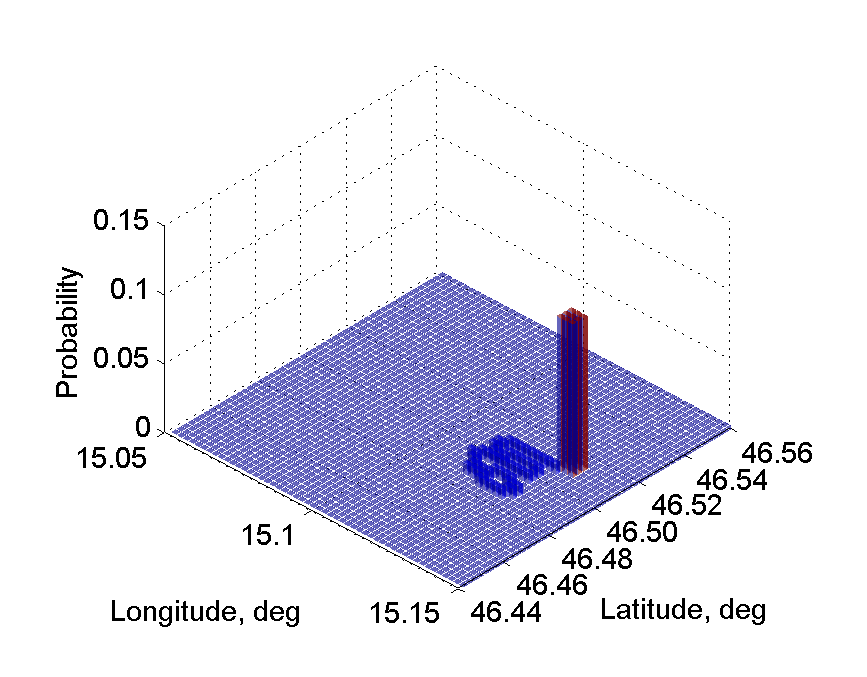
\includegraphics[scale=0.51]{Figures/Mapping_thermals_2.eps}
  \caption{Evolution of $p(X(t)\vert S(t))$ obtained by glider $\#1$.}
  \label{fig:SimPDF}
\end{figure}
%%%%%%%%%%
\begin{figure}[thp]
  \centering
  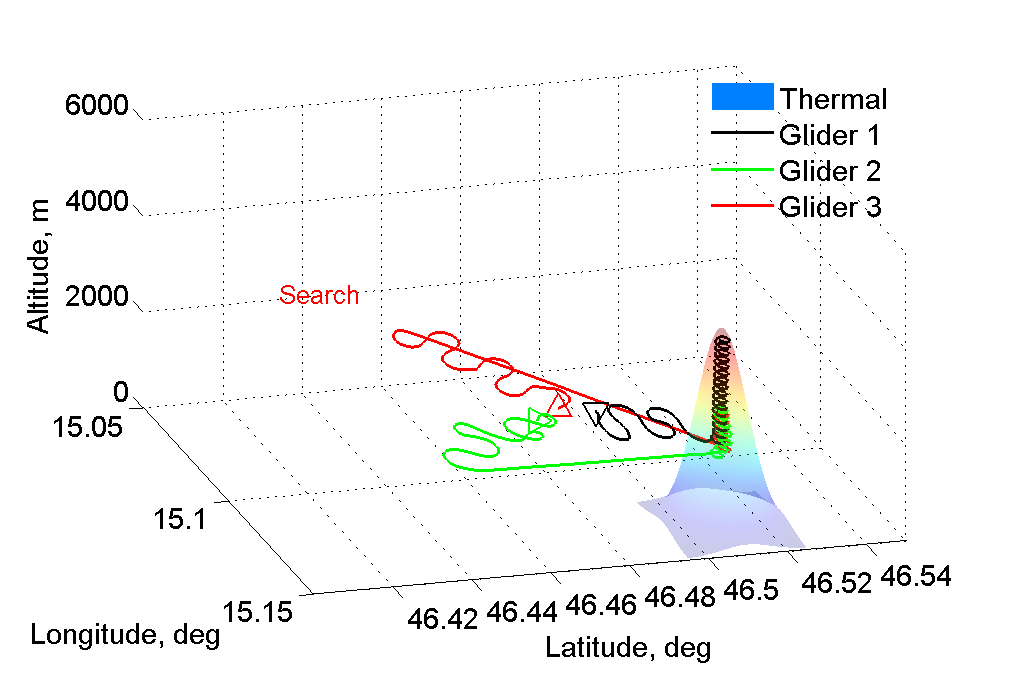
\includegraphics[scale=0.41]{Figures/paths_cooperative_flight_2.eps}
  \caption{Cooperative flight of three gliders.}
  \label{fig:CoopFlightPaths}
\end{figure}
%%%%%%%%%%
The task is to find the updraft in a bounded area and to converge to the same
thermal by utilizing the detection algorithms discussed above; the task
mimics the setup and the objectives of our first cooperative flight test of
two gliders reported earlier in \cite{AKlass_JGCD:2012}. In the demonstrated
result the prior probability density is initialized by a uniform function
over the entire area of operation. The result illustrates the evolution of
the probability density function estimated by glider $\#1$ , see the corresponding trajectories of gliders $\#2$
and $\#3$ in Fig.~\ref{fig:CoopFlightPaths}.
%, see more details on the
%simulation setup in section \ref{sec:SimEnv}.\squeezeup

\section{Simulation Environment}
\label{sec:SimEnv}
\squeezeup

To facilitate the design and verification of the designed algorithms the
project developed a realistic simulation environment that is based on
integration of MatLab/Simulink (\cite{MATLAB:2013}) capabilities with the
high-fidelity flight dynamics and atmospheric effects of the Condor soaring
simulator, see \cite{Condor:2013:Online}. Besides providing a wide
nomenclature of gliders, the networking capability of the Condor enables the
cooperative behaviors of multiple agents that is essential to the project.
The architecture of the software in the loop setup is presented in
Fig.~\ref{fig:SIL}.
%
%Since the goal is to enable autonomous soaring and exclude the manual pilot
%command, the standard software was patched with a an API (windows service)
%that enabled reading of all states of the glider in a Simulink model and
%sending of the control surface commands from the cooperative soaring
%algorithms implemented by the MatLab/Simulink models.

%%%%%%%%%%
\begin{figure}[thpb]
  \centering
  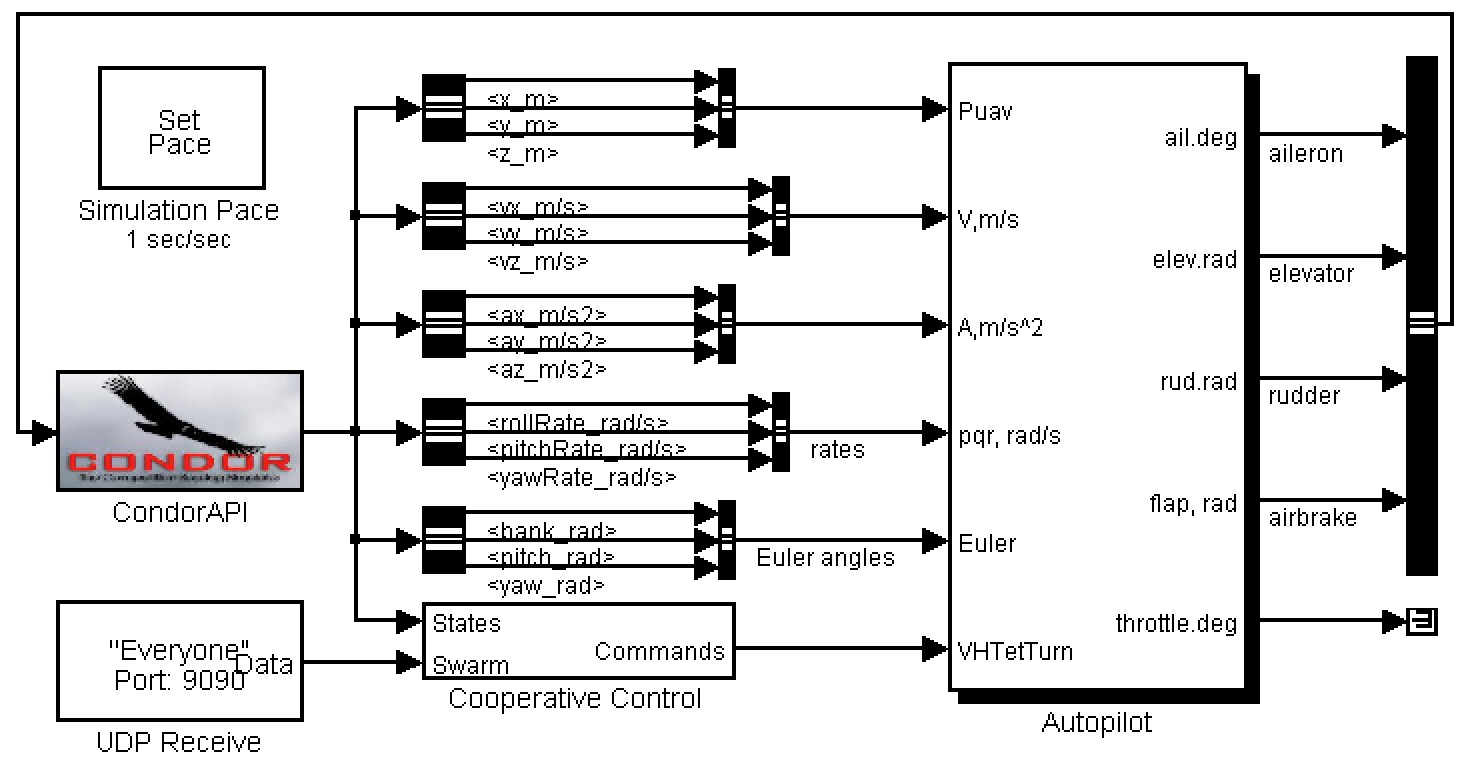
\includegraphics[scale=0.325]{Figures/SIL.eps}
  \caption{Integration of Simulink and Condor capabilities.}
  \label{fig:SIL}
\end{figure}
%%%%%%%%%%

%%%%% If this section on the API is used then include Dmitrij as a coauthor %%%%%%
%Condor API is the utility that enables the read telemetry and write commands
%functionality in the SIL environment. Condor API is implemented as a Windows
%Service and uses .NET Framework 4.0. Condor Soaring Simulator (Condor.exe)
%sends telemetry to Condor API Windows Service; CondorAPI listens for
%telemetry on CondorEndpoint. Then Condor API reads additional parameters from
%Condor process, adds those parameters to telemetry and sends to external
%endpoint (MatLab/Simulink). Also Condor API service listens for commands
%(elevator,rudder,ailerons,airbreaks) on CommandsEndpoint and executes them by
%writing to condor process memory.
%
%In a configuration where Condor software and the Simulink model are running on the same computer
%all endpoints can be configured in a single config file as follows:
%\begin{itemize}{\leftmargin=0em \itemindent=0em}
%  \item[] $<$HostSettings$>$
%    \begin{itemize}
%        \item[] $<$CondorEndpoint host="127.0.0.1"port="278"$/>$
%        \item[] $<$ExternalEndpoint host="127.0.0.1"port="279"$/>$
%        \item[] $<$CommandsEndpoint host="127.0.0.1"port="280"$/>$
%    \end{itemize}
%  \item[] $< /$HostSettings$>$
%\end{itemize}
%
%%%%%%%%%%%
%\begin{figure}[thpb]
%  \centering
%  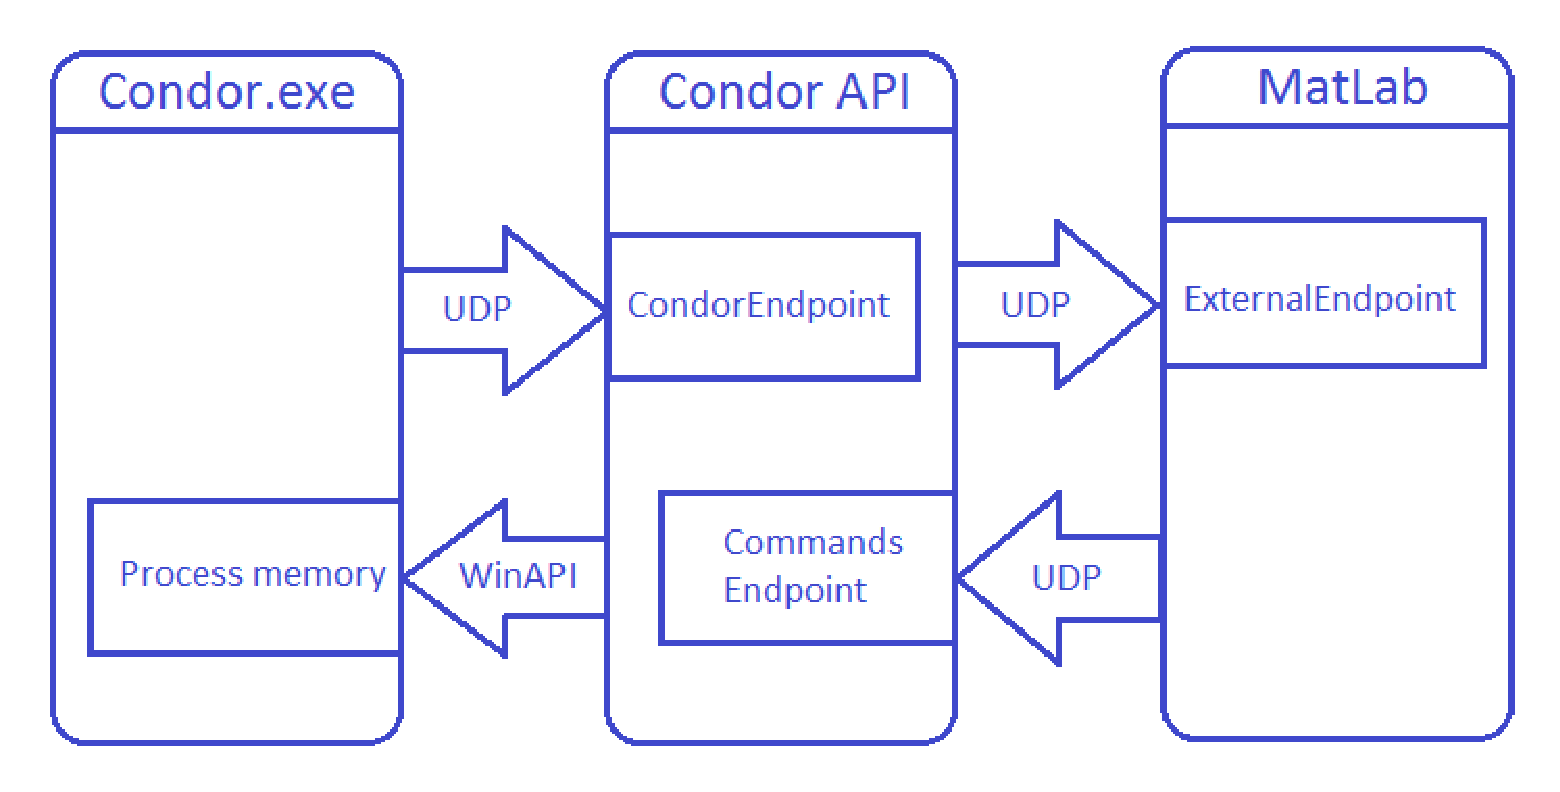
\includegraphics[scale=0.3]{Figures/API.eps}
%  \caption{Condor API architecture.}
%  \label{fig:API}
%\end{figure}
%%%%%%%%%%%

As an illustration of the achieved capabilities,
Fig.~\ref{fig:CoopFlightPaths} represents the cooperative flight of three
gliders in a simplified scenario introduced above. The gliders start their
flight simultaneously at the same altitude, and initially spend some time in
search for thermals. When glider $\#1$ detects an updraft utilizing either of
the thermal detection approaches ( see sec.\ref{subsec:SysID}), and shares
the information about the thermal, the other two gliders arrive to the same
thermal and successfully gain height. Time history of the altitude of three
cooperative gliders is presented next in Fig.~\ref{fig:CoopFlightHeight}. The
result demonstrates the benefits of collaborative strategies in harvesting the
convective updraft energy.
%%%%%%%%%%
\begin{figure}[thpb]
  \centering
  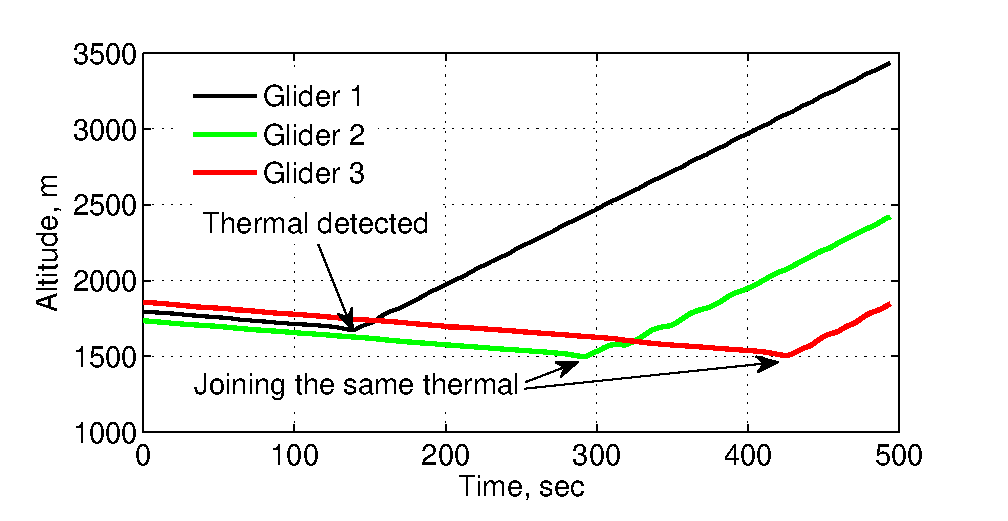
\includegraphics[scale=0.39]{Figures/Coop_gain_altitude_2.eps}
  \caption{Cooperative gain of altitude.}
  \label{fig:CoopFlightHeight}
\end{figure}
%%%%%%%%%%
\squeezeup

%\section{Future work}
%\label{sec:Future}
%The future plans include the development in two primary
%directions. First is the design of novel distributed approaches for effective
%environment sensing and energy harvesting along with the cooperative mission
%management and execution algorithms. We envision that in a typical mission
%with the goal defined by the waypoints in the area of operation, the task of
%finding an optimal route for multiple ''traveling salesman`` to visit all
%waypoints can be solved by weighting the edges of the underlying graph
%according to the proximity to the free energy sources in the area. Second is
%to develop new hardware platform with high efficiency flexible solar panels
%integrated into the skin of the glider wings and the corresponding monitoring
%and the energy management algorithms. The task is underway with expected
%first flight of a single solar powered platform to be performed in February
%2014.

\section{Conclusion}
\squeezeup
%A conclusion section is not required. Although a conclusion may review the
%main points of the paper, do not replicate the abstract as the conclusion. A
%conclusion might elaborate on the importance of the work or suggest
%applications and extensions.
The paper presents the development of convective thermal and solar energy
harvesting capability integrated onboard of multiple gliders. The
discussion details the key technologies required to integrate the energy
harvesting into a cooperative mission planning and execution environment. The
key components include the online characterization of the electrical management system,
glider properties, convective thermals detection, and the collaborative environment sensing by utilizing Bayesian estimation.

%\begin{ack}                              % Place acknowledgements here
%%The project has been supported by a number of sponsors including the NPS
%%Consortium for Robotics and Unmanned Systems Education and Research, the Army
%%Research Lab, and the "The Multidisciplinary Studies Support for USMC
%%Expeditionary Energy Office" program.
%The authors would like to mention the contribution of graduate students
%Andrew Streenan and Joshua Weiss for providing results of their final project
%and contributing to the extensive simulation research.
%\end{ack}

%\bibliographystyle{ifacconf-harvard}        % Include this if you use bibtex
\bibliography{ifacconf}           % and a bib file to produce the


%\appendix
%\section{A summary of Latin grammar}    % Each appendix must have a short title.
%\section{Some Latin vocabulary}         % Sections and subsections are supported
%                                        % in the appendices.
\end{document}
